\chapter{Introduction}
	\section{What is \Kieker?}

		\Kieker\ is a framework facilitating the monitoring and analysis of control flows, response times and generally the runtime behavior of Java applications. Normal ({}``plain) Java applications can be arranged with the framework as well as server based Java web applications. The framework itself has been developed with regard to providing an easy manageable, maintainable piece of software, which can be included uncomplicated into both, new and existing software projects. Kieker has been designed for a continuous operation, resulting in a very small overhead during the monitoring. Kieker can probe whole method calls as well as single statements (e.g. a = a + 1).\\ 
		Nearly every component of the framework can be extended and adjusted easily as necessary.

		% This is the component diagram of Kieker (the satellite).
		\begin{figure}[H]
			\begin{centering}
				\includegraphics[width=1\textwidth]{images/kiekerComponentDiagram}
			\end{centering}
			\caption{The component diagram of \Kieker}
			\label{Figure:KiekerComponentDiagram}
		\end{figure}
		
		Figure \ref{Figure:KiekerComponentDiagram} shows that the framework consists mainly of two big parts:
		\begin{itemize}
			% Both items get notify-tags because of the important information in here.
			\item \KiekerMonitoringPart\\
			This is the part which is responsible for probing, logging and recording the program behavior. Its core is the singleton class \class{MonitoringController} \notify which receives the records and stores them into different monitoring logs, like for example into files or into databases.
			\item \KiekerAnalysisPart\\
			This part is responsible for the evalution and possible visualization of the recorded information. Its core is the class \class{AnalysisInstance} \notify which manages the lifecycle of the readers and all plugins which shoud analyze the stored informations.
		\end{itemize}
		Both parts are composed of subcomponents which can just be used or extended as well with own classes. The rough interaction between the components is described in Figure \ref{Figure:KiekerCommunicationDiagram} but will be explained furthermore in the course of this tutorial.

		% This image shows the communication diagram of the different components.
		\begin{figure}[H]
			\begin{centering}
				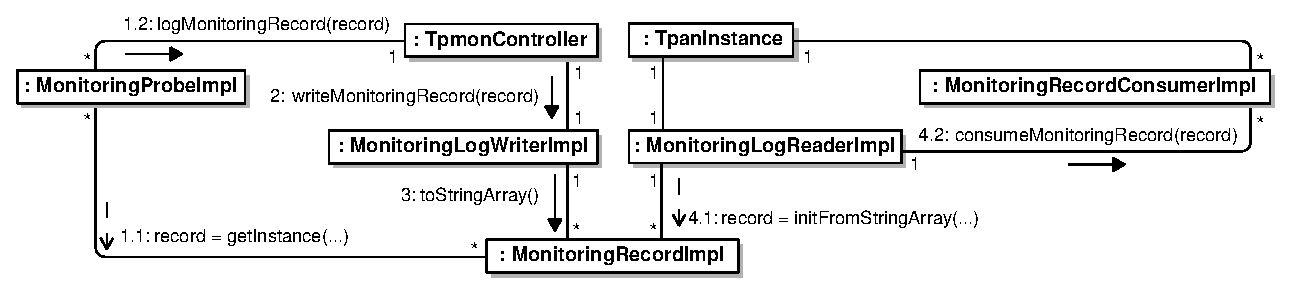
\includegraphics[width=1\textwidth]{images/kiekerCommunications-revisedReArranged-woMonitoringLog-bw}
			\end{centering}
			\caption{The communication diagram of \Kieker}
			\label{Figure:KiekerCommunicationDiagram}
		\end{figure}
		
		% Notify-tag because it is explained how Kieker works.
		\notify The monitoring probes create the monitoring records and deliver them to the monitoring controller. The monitoring controller uses the monitoring log writers to persist the given records which can later be read by a monitoring log reader who creates a monitoring record again. These records can then be used by the consumers in nearly every way.

	\section{Features}
	% This part has to be filled!
	
	\section{The purpose of this tutorial}
		% Short explanation what the tutorial will show now.
		This tutorial will take a closer look at both, the \KiekerMonitoringPart - and the \KiekerAnalysisPart-part. It will be described on the one hand how \KiekerMonitoringPart  can be used to mark parts of the own sourcecode for \Kieker\  and to let them run under surveilance, so that the recorded informations can be persisted somewhere and on the other hand \KiekerAnalysisPart will be used for processing the recorded data.\\
		Before this tutorial goes deeper into the single parts of the framework, it shows how to create and execute a simple example.